%!TEX root = ../../clcxsj.tex

\chapter{ \cs 开发环境与程序基础}

我们学习过C语言,有一定的计算机编程基础。C语言是功能强大的高效
程序设计语言,但在现代的软件开发中特别是 Window 界面程序开发中的效率太低了。
Microsoft推出的.Net Framwork在新版Windows中越来越多的进行了预安装,
 \cs 语言面向对象、语法优美、功能强大、开发效率高,应用也越来越广泛。
因此我们将从C语言程序设计转向 \cs 程序设计语言,
学习更多的现代程序设计方法,满足现代测绘大数据的处理与算法编写需求。

\section{ \cs  开发环境与工具}

\subsection{ \cs  开发环境}
Microsoft Visual Studio 是微软出品的经典的集成开发环境(Integrated Development Environment,
简称IDE),也是 \cs 语言开发的经典工具,目前常用的版本为2017、2019、2022版,最新版本为2022版。
本课程将使用 Microsoft Visual Studio Community 2022。

安装好 Microsoft Visual Studio Community 222后,基本上 \cs  的开发环境就准备好了。

\subsection{版本控制与源代码管理}
git 软件是目前最流行的开源分布式版本控制软件,也称为软件业的时光机。
在我们的软件编写过程中,将使用它进行源代码管理。

TortoiseGit 是 git 的图形化客户端软件,开源软件,支持中文等语言。

Visual Code 与  Notepad++ 是开源的文本编辑软件,功能比微软自带的记事本强大的多,
在程序编写中可以快速地查看与修改源代码。


\section{第一个 \cs  程序}

\subsection{单个 \cs  源代码文件的编写}
我们用 \cs 语言编写经典的C语言入门程序Hello World。打开 Visual Code 或 Notepad++,
首先将文件保存为HelloWorld.cs文件,在其中输入以下代码:

%  [caption={HelloWorld源代码}, label=srcHelloWorld]
\begin{lstlisting}
// HelloWorld.cs
using System;

namespace HelloWorld
{
	class Program
	{
		static void Main(string[] args) 
		{
			Console.WriteLine("Hello World!");
		}
	}
}
\end{lstlisting}

\subsection{单个 \cs  源代码文件的编译与执行}
点击开始菜单中的 Developer Command Prompt for VS 2022 或 Developer PowerShell for VS 2022,
切换到 HelloWorld.cs 文件所在的文件夹,输入: csc HelloWorld.cs 将编译生成 HelloWorld.exe 
可执行程序。

再输入:HelloWorld,程序执行输出:Hello World!

以上命令中csc为 \cs 语言的编译器,作用为检查 \cs 源代码文件中的语法,将其翻译成 .Net Framwork 
能识别的中间语言(Microsoft Intermediate Language,简称为IL),
最后在.Net Framwork的公共语言运行库(Common Language Runtime,简称为CLR)支持下解释为可执行的计算机命令。

整个过程如图\ref{fig:BuildHelloWorld}所示。
\begin{figure}[htbp]
	\centering
	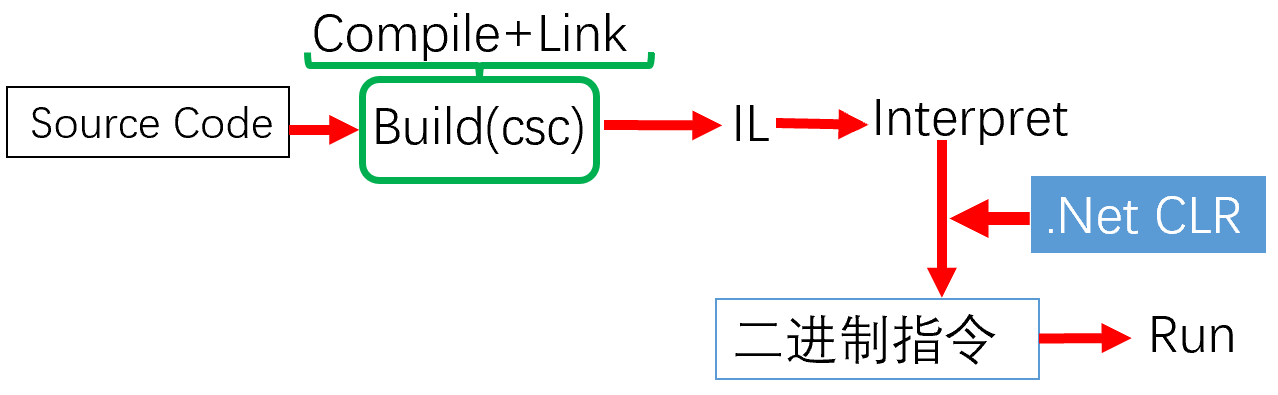
\includegraphics[scale=0.8]{chapter/csenv/BuildHelloWorld.png}
	\caption{HelloWorld程序构建过程}
	\label{fig:BuildHelloWorld}
\end{figure}

\subsection{使用IDE编辑、编译与运行 \cs 程序}
一个程序除了源代码之外,还有图标、图片、配置信息等等文件,源代码文件也可能有多个,
用以上方式编辑、构建可执行文件太复杂了,这时使用IDE的效率会更高。

用Visual Studio 生成一个HelloWorld 控制台(Console)项目,
在Program.cs文件中会自动生成以上代码,点击工具栏上的运行按钮,即可编译运行程序。

使用 Visual Studio 2022 生成以上项目时,如果不勾选``不使用顶级语句'',
则只会在Program.cs文件中生成一个语句:

% 顶级语句  [caption={HelloWorld源代码}, label=srcHelloWorld]
\begin{lstlisting}
Console.WriteLine("Hello World!");
\end{lstlisting}

这是 .NET 6 项目的生成顶级语句(top-level statements)的新模板。相当于去掉了
using、namespace以及默认的类Program与默认的Main函数,这些由编译器在编译时自动生成。
具体请参看\href{https://docs.microsoft.com/en-us/dotnet/core/tutorials/top-level-templates}{微软官方文档}。

在顶级语句的文件中,整个文件 Program.cs 的内容都相当于 Main 函数的内容,不能在其中编写除语句之外的内容。

\subsection{Visual Studio文件组织形式分析}
在文件资源管理器中打开HelloWorld项目,文件组织形式如图\ref{fig:HelloWorldProj}所示:

\begin{figure}[htbp]
\centering
\subfloat[解决方案]
{
	\label{fig:HelloWorldProj-a}
	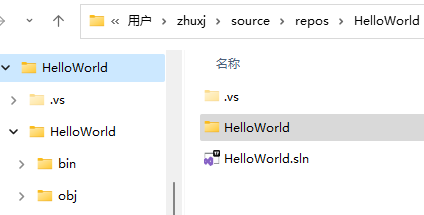
\includegraphics[scale=1]{chapter/csenv/HelloWorldProj1.png}
}
\hspace{20pt}%
\subfloat[项目]
{
	\label{fig:HelloWorldProj-b}
	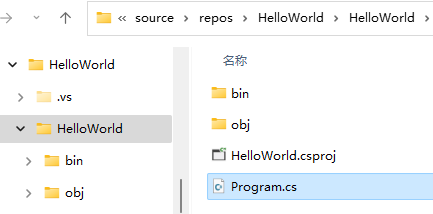
\includegraphics[scale=1]{chapter/csenv/HelloWorldProj2.png}
}
\caption{HelloWorld程序文件结构}
\label{fig:HelloWorldProj}
\end{figure}

图\ref{fig:HelloWorldProj-a} 为解决方案的文件夹,系统在生成解决方案时,
会根据工程名(或解决方案名)自动创建一个文件夹,如本例中的HelloWorld,
并在文件夹中创建一个解决方案的文件HelloWorld.sln与工程文件夹HelloWorld。

文件HelloWorld.sln为文本文件,可以用 Visual Code 或 Notepad++打开,
其内容如下:

\begin{lstlisting}
Microsoft Visual Studio Solution File, Format Version 12.00
# Visual Studio Version 17
VisualStudioVersion = 17.0.31612.314
MinimumVisualStudioVersion = 10.0.40219.1
Project("{FAE04EC0-301F-11D3-BF4B-00C04F79EFBC}") = "HelloWorld", "HelloWorld\HelloWorld.csproj", "{770A121E-217D-435D-AAB7-2EDE7EC5A7C9}"
EndProject
Global
	......省略......
EndGlobal
\end{lstlisting}

第5行中说明了HelloWorld项目的相关信息。

图\ref{fig:HelloWorldProj-b}为项目HelloWorld的文件夹,
该文件夹中有一个工程文件HelloWorld.csproj,
一个  \cs  源代码文件Program.cs、两个文件夹bin与obj,
bin用于存放最后生成的可执行文件,obj缓存系统中间文件。

文件HelloWorld.csproj内容如下:
\begin{lstlisting}
<Project Sdk="Microsoft.NET.Sdk">

	<PropertyGroup>
		<OutputType>Exe</OutputType>
		<TargetFramework>net5.0</TargetFramework>
	</PropertyGroup>

</Project>
\end{lstlisting}

这个文件记录了项目的生成类型与运行目标框架。

从以上看出,Visual Studio 是用文件夹与文件的形式来组织管理项目的。
一个项目由多个源代码文件、资源文件等组成,经过编译链接最终生成为程序集。
程序集通常具有文件扩展名 .exe 或 .dll,具体取决于它们是实现应用程序 (application) 还是实现库 (library)。

一个或多个项目组成一个解决方案(Solution)。

一个项目的构建过程如图\ref{fig:BuildProject}所示:
\begin{figure}[htbp]
	\centering
	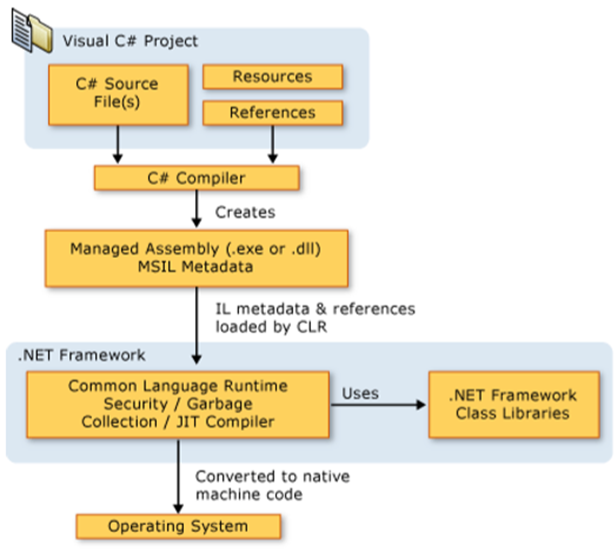
\includegraphics[scale=1.4]{chapter/csenv/BuildProject.png}
	\caption{项目构建过程}
	\label{fig:BuildProject}
\end{figure}



\section{ \cs  程序结构分析}

分析以上 \cs 示例中的HelloWorld.cs源代码可以看出,
  \cs  程序中的一些关键概念:
 \begin{itemize}
	 \item using指令
	 	
	 \item 命名空间 (namespace)
	 \item 类程序 (class)
	 \item 类的静态成员函数(static)
	 \item Console类(控制台类)
 \end{itemize}

  \cs  程序由一个或多个源代码文件组成。每个源代码中声明类,类包含成员,并且可按命名空间进行组织。
 类的成员有字段 (field)、方法、函数、属性和事件等。
 
\section{扩展:从C走向 \cs }

\subsection{Client/Server程序设计模式}
现代软件往往是多人协作开发的成果,单个人进行大型软件的开发是比较少的。
在软件开发中需要遵循软件工程的组织原则,寻求代码的可复用性、可测试性
、可阅读性与可维护性。在学习编程时我们首先应该改掉以下三个不良编码习惯:

改变C语言中将代码直接写入main函数中的习惯;

改变在 \cs 语言中将代码直接写入Main函数中的习惯;

改变在UI(WinForm或WPF或其它的界面)中直接写入逻辑算法代码的习惯。

以上三种形式的代码书写处的Main函数或界面调用函数我们可以称为Client,我们编写的逻辑算法代码可以称为
Server。试想如果我们去商场买东西,我们就是Client,提供需求;商场就是Server,提供服务。
如果我们要买一只圆珠笔,也许我们只需简单的告诉商场人员,然后付钱拿笔走人就行了。但如果
商场要让我们自己去仓库里找笔、查价钱、再在商场登记簿上登记库存等等一些动作,
你想想会是怎么样的一种结果?买只笔都要把我们累死了。

这说明了什么呢?提供服务功能的商场应该对有功能需求的客户简化和屏蔽各种复杂的中间环节。
在软件开发时同样如此,我们的main或Main函数或UI处的代码应该简洁,
基本上只是调用各个功能算法而已。

如果我们像以上这三种方式组织代码,将会带来一系列的问题,
尤其在团队开发与多人协作时代码不能复用,不能进行 unit test (单元测试)、
不能用git工具(著名的源代码管理工具)进行源代码的自动合并。
软件系统稍微复杂一点,我们的开发就会面临不可控甚至失败的危险。

万丈高楼从地起,因此,在学习编程时首先我们要有Client/Server模式意识,
要遵循界面与算法相分离的原则进行程序设计。

\subsection{从面向过程走向面向对象的程序设计 }

良好的面向过程设计程序设计程序是可以很好的转向面向对象的程序设计的,我们将从一个简单的
C程序开始设计结构较为良好的C代码,再将其用面向对象的 \cs 进行实现。从中体会面向过程与
面向对象的程序设计方法的不同。

 \subsubsection{面向过程的C代码示例}

在测绘专业中我们经常与测量点打交道,因此我们定义一个点Point(测点除了它的坐标x,y和高程z之外,还需至少有点名),
 另外我们定义一个简单的为大家所熟知的圆Circle,来使用点Point定义它的圆心,并实现判断两圆是否相交,
 计算圆的面积和周长等功能。代码如下所示:

\lstinputlisting[language=C,
        % caption={C代码示例}, label=Ch01Ex01,
        firstline=1, lastline=40]
        {./chapter/csenv/Ch01Ex01/Ch01Ex01/Ch01Ex01.cpp}

\subsubsection{对C代码的解释}
代码中的11和16行定义结构体时使用了 typedef,这样在标准C中再定义Point类型或Circle类型时可以避免
在其前面加关键词struct。

第24-26行计算圆的面积,传入了圆的指针,这是C及C++中传递自定义数据类型的常用的高效方式。
由于计算的圆面积会保存在结构体Circle中的area中,所以函数不需要返回值,返回值定义为void。

第29-33行为计算两点的距离,由于该函数不会修改p1、p2两个Point内的任何成员,故应该将这两个指针
定义为const类型,防止函数内部无意或故意的修改。

同理第36-39行判断两圆是否相交,由于该函数不会修改c1、c2两个圆内的任何成员,也应将这两个指针
定义为const类型。

第37行由于Distance函数的参数需要两个Point指针类型的参数,尽管c1与c2均为指针,但c1->center与
c2->center不是指针,所以需要在其前用取地址符 \& 。

第38行的关系运算符本身的运算结果就为bool型,故不需要进行if、else类型的判断。

相应的main函数测试代码如下:

\lstinputlisting[language=C, 
% caption={Client作用的C main函数}, label={code:Ch01Ex01main},
firstline=41, lastline=65]
{./chapter/csenv/Ch01Ex01/Ch01Ex01/Ch01Ex01.cpp}

程序的运行结果如下:
\begin{verbatim}
Circle1 的面积 = 20106.192983
Circle1 与 Circle2 是否相交 :是
\end{verbatim}


\subsection{与C相对应的 \cs 代码}

将以上代码相对应的C代码直接翻译为 \cs 代码为:

\lstinputlisting{./chapter/csenv/Ch01Ex02/Ch01Ex02/Circle.cs}
% \caption{由C转换为 \cs 的示例代码}\label{code:Ch01Ex02}

由以上 \cs 代码可以看出与C代码的不同。这是因为 \cs 语言是纯面向对象语言的缘故。

程序或软件的基本概念是:程序 = 数据结构 + 算法。在以上C或 \cs 代码中,Point和Circle
都可以看作是数据结构,计算两点距离和圆的面积或判断两圆是否相交都可以看作是算法。
在C语言中,数据结构和算法是分离的,尽管函数的参数是数据结构,但函数并不属于数据结构。
在 \cs 中则不同,数据结构用class定义,则数据与算法都属于同一个class。

计算两点距离的函数设计为Point类的一个方法,可以看作是计算当前点与另一个点的距离,
因此函数的参数就只有一个Point p2,另一个自然是this(当前类本身)了。

同样的道理圆的面积计算也不需要参数了(可以想象为计算知道自己的半径,计算自己的面积
并存入自己的成员变量中了)。判断两圆是否相交也可以看作是判断当前圆与另一个圆Circle c2
是否相交了,股只需要一个参数。

相应 \cs 的Main函数测试代码如下:

\lstinputlisting{./chapter/csenv/Ch01Ex02/Ch01Ex02/Program.cs}
% \caption{Client化的 \cs Main函数}\label{code:Ch01Ex02Main}

程序的运行结果如下:
\begin{verbatim}
Circle1的面积=20106.1929829747
Circle2的面积=38013.2711084365
Circle1与Circle2是否相交:是
\end{verbatim}

\subsection{面向对象的 \cs 代码}
上面的 \cs 不符合面向对象的软件设计原则(违背封装、继承与多态中的封装原则),且在Main函数中,如果由于
疏漏忘记第30行或33行对圆的面积进行计算,圆c1或c2将不会有正确的面积。

因此,我们将其优化。首先对Point类进行封装,将其字段定义为private,
用属性方法将其向外暴露接口,相应的 \cs 代码为:

\lstinputlisting[firstline=7, lastline=32]{./chapter/csenv/Ch01Ex03/Ch01Ex03/Circle.cs}

以上是用 \cs 的属性对private字段的进行简单的封装,也可以写成如下形式:
\begin{lstlisting}
public string Name { get ; set ; }
public double X { get ; set ;}
public double Y { get ; set ; }
public double Z {get ; set ;}
\end{lstlisting}

为了简化Main函数对Point类的调用及对其各字段值的初始化,我们定义构造函数如下:
\lstinputlisting[firstline=33, lastline=47]{./chapter/csenv/Ch01Ex03/Ch01Ex03/Circle.cs}

同样道理,也应对Circle进行封装,将其各个字段定义为private,
并用属性方法将其向外简单的暴露接口,相应的 \cs 代码为:

\lstinputlisting[firstline=59, lastline=74]{./chapter/csenv/Ch01Ex03/Ch01Ex03/Circle.cs}

圆心Center只是简单的封装,圆的半径则不同。由圆的特性知,当圆的半径确定,
其面积与周长也就确定了。为了计算的高效,封装时,当圆的半径值发生改变时,
就需要重新计算圆的面积,确保面积的正确性。

由于圆的面积只与圆的半径有关,我们不需要在其他的情况对圆的面积进行修改,
因此封装的 \cs 代码为:

\lstinputlisting[firstline=75, lastline=80]{./chapter/csenv/Ch01Ex03/Ch01Ex03/Circle.cs}

在此我们去掉了属性Area中的set语句,并将area成员定义为了private,使外部无法修改area的值,
来保证圆的面积Area的正确性。

还有一个地方可能会修改圆的半径,就是圆的初始化时,因此圆的构造函数应定义为:

\lstinputlisting[firstline=83, lastline=89]{./chapter/csenv/Ch01Ex03/Ch01Ex03/Circle.cs}

为确保在半径r的值发生改变后能重新计算圆的面积和周长,此处赋值给半径属性R。

完整的优化后的 \cs 代码如下:
\lstinputlisting{./chapter/csenv/Ch01Ex03/Ch01Ex03/Circle.cs}

代码中由于计算圆的面积将会在属性R中和构造函数中调用,
我们将其定义为函数CalArea供多次复用,
并将可访问性定义为private供内部使用。

相应 \cs 的Main函数测试代码如下:

\lstinputlisting{./chapter/csenv/Ch01Ex03/Ch01Ex03/Program.cs}

由优化后的 \cs 代码可以看出Main十分简洁。

\section{作业}
\begin{enumerate}
\item 请完成示例中的圆的周长计算功能;
\item 请试着完成多段线Polyline的面积与长度计算功能(提示:多段线是点序的集合);
\item 请试着完成多边形Polygon的面积与长度计算功能。

提示:多边形面积计算公式为:

$$S=\frac{1}{2}\sum_{k=1}^{6}{(x_k y_{k+1} - x_{k+1} y_k)}$$

多边形的顶点坐标依次为
$p_1(-1,0), p_2(2,3), p_3(4,2), p_4(4,4),p_5(6,8),p_6(-2,5)$,
则依上式计算该多边形面积为28.
\end{enumerate}
